\chapter{Preliminary Results}
\label{ch:results}

\section{Deterministic transport}

\subsection{Verification and analysis of discretization scheme}

I found that the MB-SCB scheme is unconditionally stable over $\mu \in [-1, 1]$. While experimenting with this method we did find that, under some conditions, it can produce negative fluxes; however, the negative flux oscillations were critically damped and dissipated with time.

I initially implemented MMS in a mono-energetic problem slab wall problem with $L=1$cm, $\Sigma$=0.5/cm, $t_0=0$s, $\Delta t = 0.1$s, $\Delta x=0.01$cm, $v=5$cm/s, $\Sigma_s=0.1$/cm, $\psi_0=\psi_m(t=0,x,\mu)$, $\psi_{x=0}=\psi_m(t,x=0,\mu)$, $\psi_{x=L}=\psi_m(t,x=L,\mu)$, in S$_{32}$.
All presented numerical investigation used a convergence tolerance of \num{1e-9} and controlled for false convergence using an on the fly estimate of spectral radius.
Figure \ref{fig:mms_sol} shows the manufactured and solver solutions matching through time.
Work is ongoing to extend this to a multi-group simulation and to use the manufacture solution to show convergence rate.


\begin{figure}[h!]
    \centering
    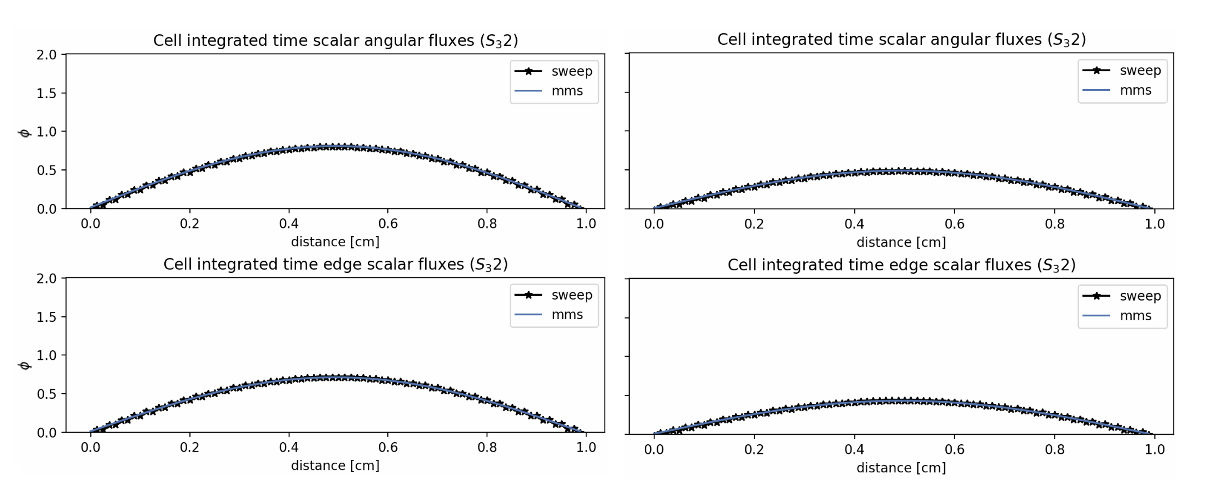
\includegraphics[width=.75\textwidth]{figures/results/mms_sol.png}
    \caption{The manufactured and solver solutions thru time.}
    \label{fig:mms_sol}
\end{figure}

%A bug exists somewhere in the current code that prevents the use of the MMS solution to also confirm order of convergence of the discritization scheme.
To verify the order of convergence of the spatial discritization an over resolved solution (at $\Delta x=\num{1e-4}$) from the solver is generated.
Error is compared at the midpoint which discritization chosen such that the midpoint is always in the same location.
Figure \ref{fig:conv_rate} shows the convergence over various choices of $\Delta x$ and shows that the scheme is second order.
Work is ongoing to confirm the order of time discritization scheme using this method.

\begin{figure}[h!]
    \centering
    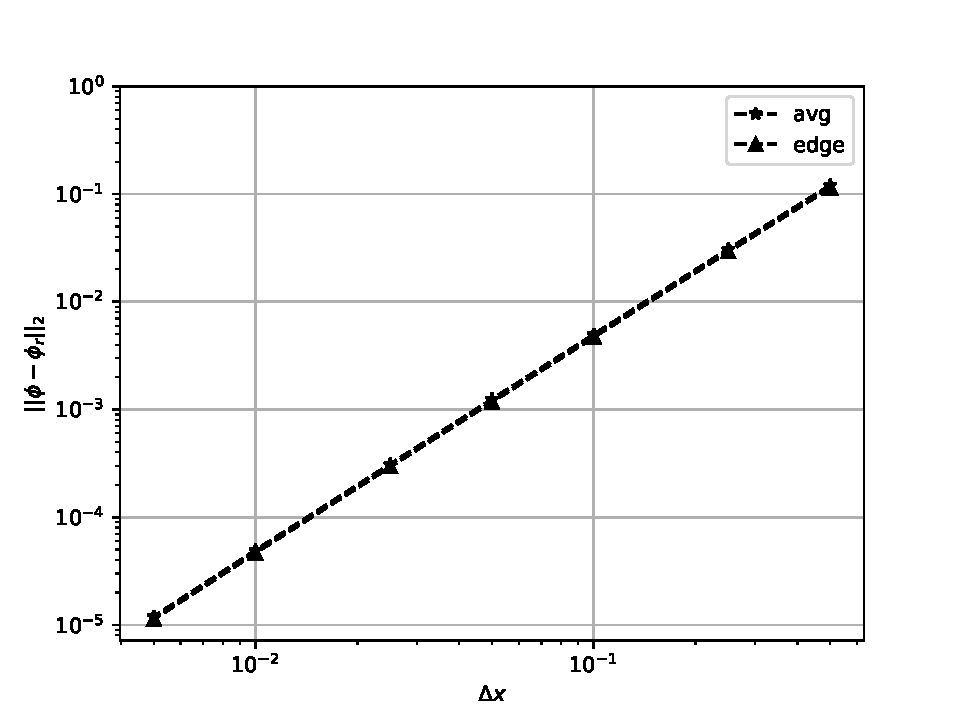
\includegraphics[width=.5\textwidth]{figures/results/convergance_rate.pdf}
    \caption{Spatial convergence rate of the discritization scheme using an over resolved $\phi_r$ solution to scalar flux from the solver.}
    \label{fig:conv_rate}
\end{figure}


\subsection{Performance Results}

Rosa, Warsa, and Perks~\cite{rosa_cellwise_2013} describe a test problem they used to validate Fourier analysis of their 2D steady state solver.
I adapt it to the 1D time dependent regime and use it to conduct preliminary performance evaluations.
Figure \ref{fig:rosa_test} shows a simple slab wall problem with vacuum boundary conditions and table \ref{table:rosa_test} lists the material data and solver parameters.
The initial condition is $\psi_{t=0} = 0$, and the time step $\Delta t = 0.1$ s.
Future work might explore more complex problems either with more groups or with material heterogeneity.

\begin{figure}[h!]
    \centering
    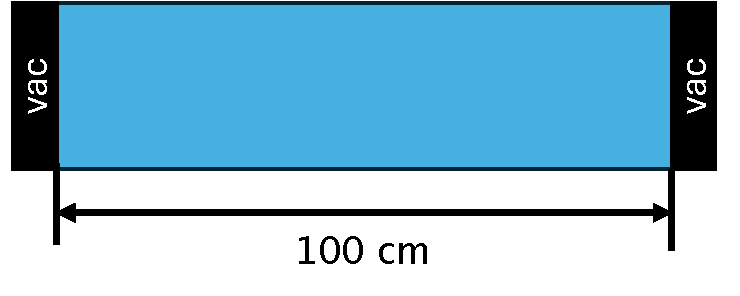
\includegraphics[width=.4\textwidth]{figures/results/rtest.pdf}
    \caption{Rosa test problem}
    \label{fig:rosa_test}
\end{figure}

\begin{table}[!htb]
  \centering
  \caption{Rosa test problem material data and simulation parameters.}
  \begin{tabular}{c c c c c c  } \hline 
    Property & Group 1 & Group 2 & units \\ \hline
    $\Sigma$ & 1.5454 &  0.45468 & cm$^{-1}$  \\
    $\Sigma_{s,g\rightarrow g}$  & 0.61789 &  0.0072534 & cm$^{-1}$  \\
    $\Sigma_{s,g'\rightarrow g}$  & 0.38211 &  0.92747 & cm$^{-1}$ \\
    $Q$ & 1 & 1 & cm$^{-3}$s$^{-1}$\\
    $v$ & 1 & 0.5 & cm s$^{-1}$ \\
    \hline
  \end{tabular}
  \label{table:rosa_test} 
\end{table}


Figure~\ref{fig:perf} at left compares the wall clock runtime of OCI (in black) and SI (in blue) over various selections of MFP (controlled via $\Delta x$ spatial discretization) and quadrature orders.
The total time to convergence was collected on the third time step to allow the GPUs to "spin up" with the initial iteration guess being 0 at every time step.
In normal compute mode this would be done with the solution from the previous time step.
Again note that the runtimes presented here are the on-GPU time in the convergence loops (see appendix \ref{app:therefore}).
The total cross section used in the MFP scale is the limiting value (the smallest) from group 2 (see Table~\ref{table:rosa_test}).
SI increases linearly as the cells get optically thinner.
The number of iterations required to converge the solution is the same but the size of the solution is getting larger.
SI only has $N_{\text{angle}}$ of $4\times 4$ systems to solve at any given moment so the amount of serial work increases with the number of cells (by decreasing $\Delta x$).
However as we increase quadrature order the runtime performance of SI actually improves as more degrees of freedom are more readily parallelized by the solvers.

\begin{figure}[h!]
    \centering
    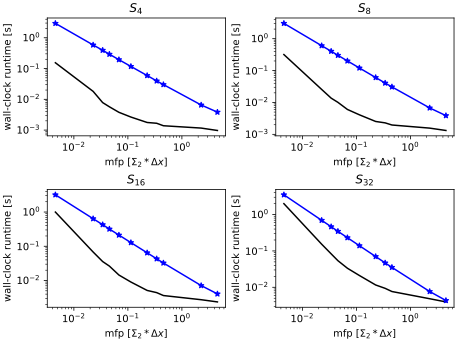
\includegraphics[width=.49\textwidth]{figures/results/runtime.png}
    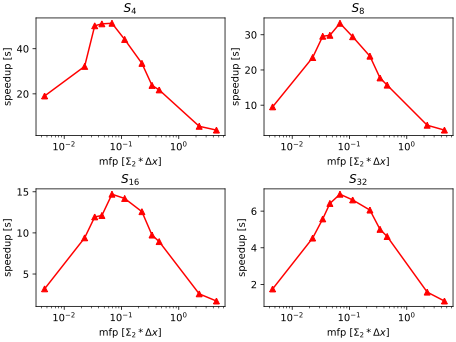
\includegraphics[width=.49\textwidth]{figures/results/speedup.png}
    \caption{Wall clock runtime of OCI black and SI red (left) and speedup (right) of Rosa et al.~\cite{rosa_cellwise_2013} test problem over choice of mean free path in various quadrature orders}
    \label{fig:perf}
\end{figure}

OCI runtime in this problem are more complex.
The degrees of freedom that can be parallelized increases with the number of cells (by decreasing $\Delta x$) however the spectral radius degrades dramatically as cells get thinner.
OCI requires more iterations to converge the solution but those iterations can be done faster on the GPU.
For OCI there seems to exist an inflection point where the method goes from increasing sub-linearly to super-linearly.
For this problem it seems to fall around mfp$=0.1$ where there are enough cells to saturate the GPU before the thin limit.

Figure \ref{fig:perf} at right shows the speedup of OCI over SI for that same problem. 
The previously mentioned optimal spot can now be seen as a definite peak around MFP$=0.1$.
The peak move slightly depending on the number of angles in quadrature.
I believe this is a feature of the \texttt{strided\_batched} solvers which can behave differently based on the dimension of the underlying matrices\cite{rocsolver}.
In smaller quadrature orders the speedup is the greatest with OCI being about 45 times faster then SI.
As more angles are added to quadrature the speed-up of OCI over SI shrinks as SI is better able to parallelize with more degrees of freedom in angle.
This confirms my previous investigations \cite{morgan2023oci} and Rosa et al.~\cite{rosa_cellwise_2013} results, that parallelizing over the largest dimension is advantageous to computation on GPU.
These conclusions provide insight into research questions 1 and 2.
%add further conclusions

\subsection{Time dependent iterative results}

To explore how time discretization impacts the convergence of OCI and SI we again use with the Rosa test problem.
Figure \ref{fig:time_desc} shows the number of iterations required to converge using both iterative schemes varying the time step, at various selections of $\Delta x$.
Again we observe that SI behaves independently of the MFP (and $\Delta x$) so the blue curve is the same on every plot.
SI does see improved convergence rate with respect to smaller time discretizations which we believe is due to improvements from the scattering ratio ($c=\Sigma_s/\Sigma$).
OCI improves with both larger choices of MFP (due to a-syncronisty) and smaller times steps due to both improvments to scattering ratio (as in SI) but now additional do to increased cellular opacity.
In fact the rate of improvement of the convergence rate actually increases in the thin limit.
This confirms our hypotheses from observations of the spectral radius, that for smaller time steps OCI converges more rapidly, especially for problems in the thin limit.
These conclusions go to answer research question 3.
% effectivaly time dependence is an accleration scheme for OCI

\begin{figure}[h!]
    \centering
    \caption{Iteration count of OCI and SI to converge the Rosa problem over various choices of $\Delta t$ and $\Delta x$}
    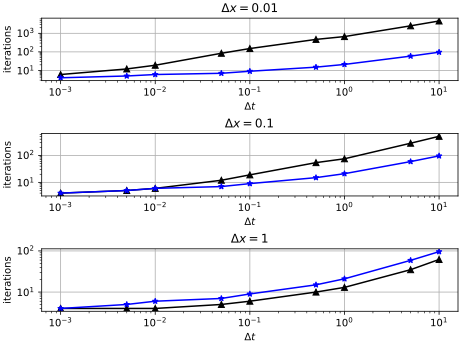
\includegraphics[width=.5\textwidth]{figures/results/time_desc.png}
    \label{fig:time_desc}
\end{figure}

\section{Monte Carlo Methods}

\subsection{MC/DC performance results}

To compare MC/DC to another Monte Carlo neutronics software package, we use a time-dependent version of the Kobayashi dog-leg void-duct problem \cite{Kobayashi2001, variansyah_mc23_mcdc}.
Figure \ref{koby-problem} at left shows the void duct and the location of the neutron source at the opening of the duct.
The initial condition is zero flux everywhere.
Radiation moves down the void quickly and then penetrates into the walls of the problem.
Figure~\ref{koby-problem} at right shows the duct clearly with the scalar flux solution in a time-averaging window of 10 s at somepoint time from MC/DC and OpenMC \cite{romano_openmc_nodate} (an open-source code written in \texttt{C++}) .

\begin{figure*}[h]
    \centering
    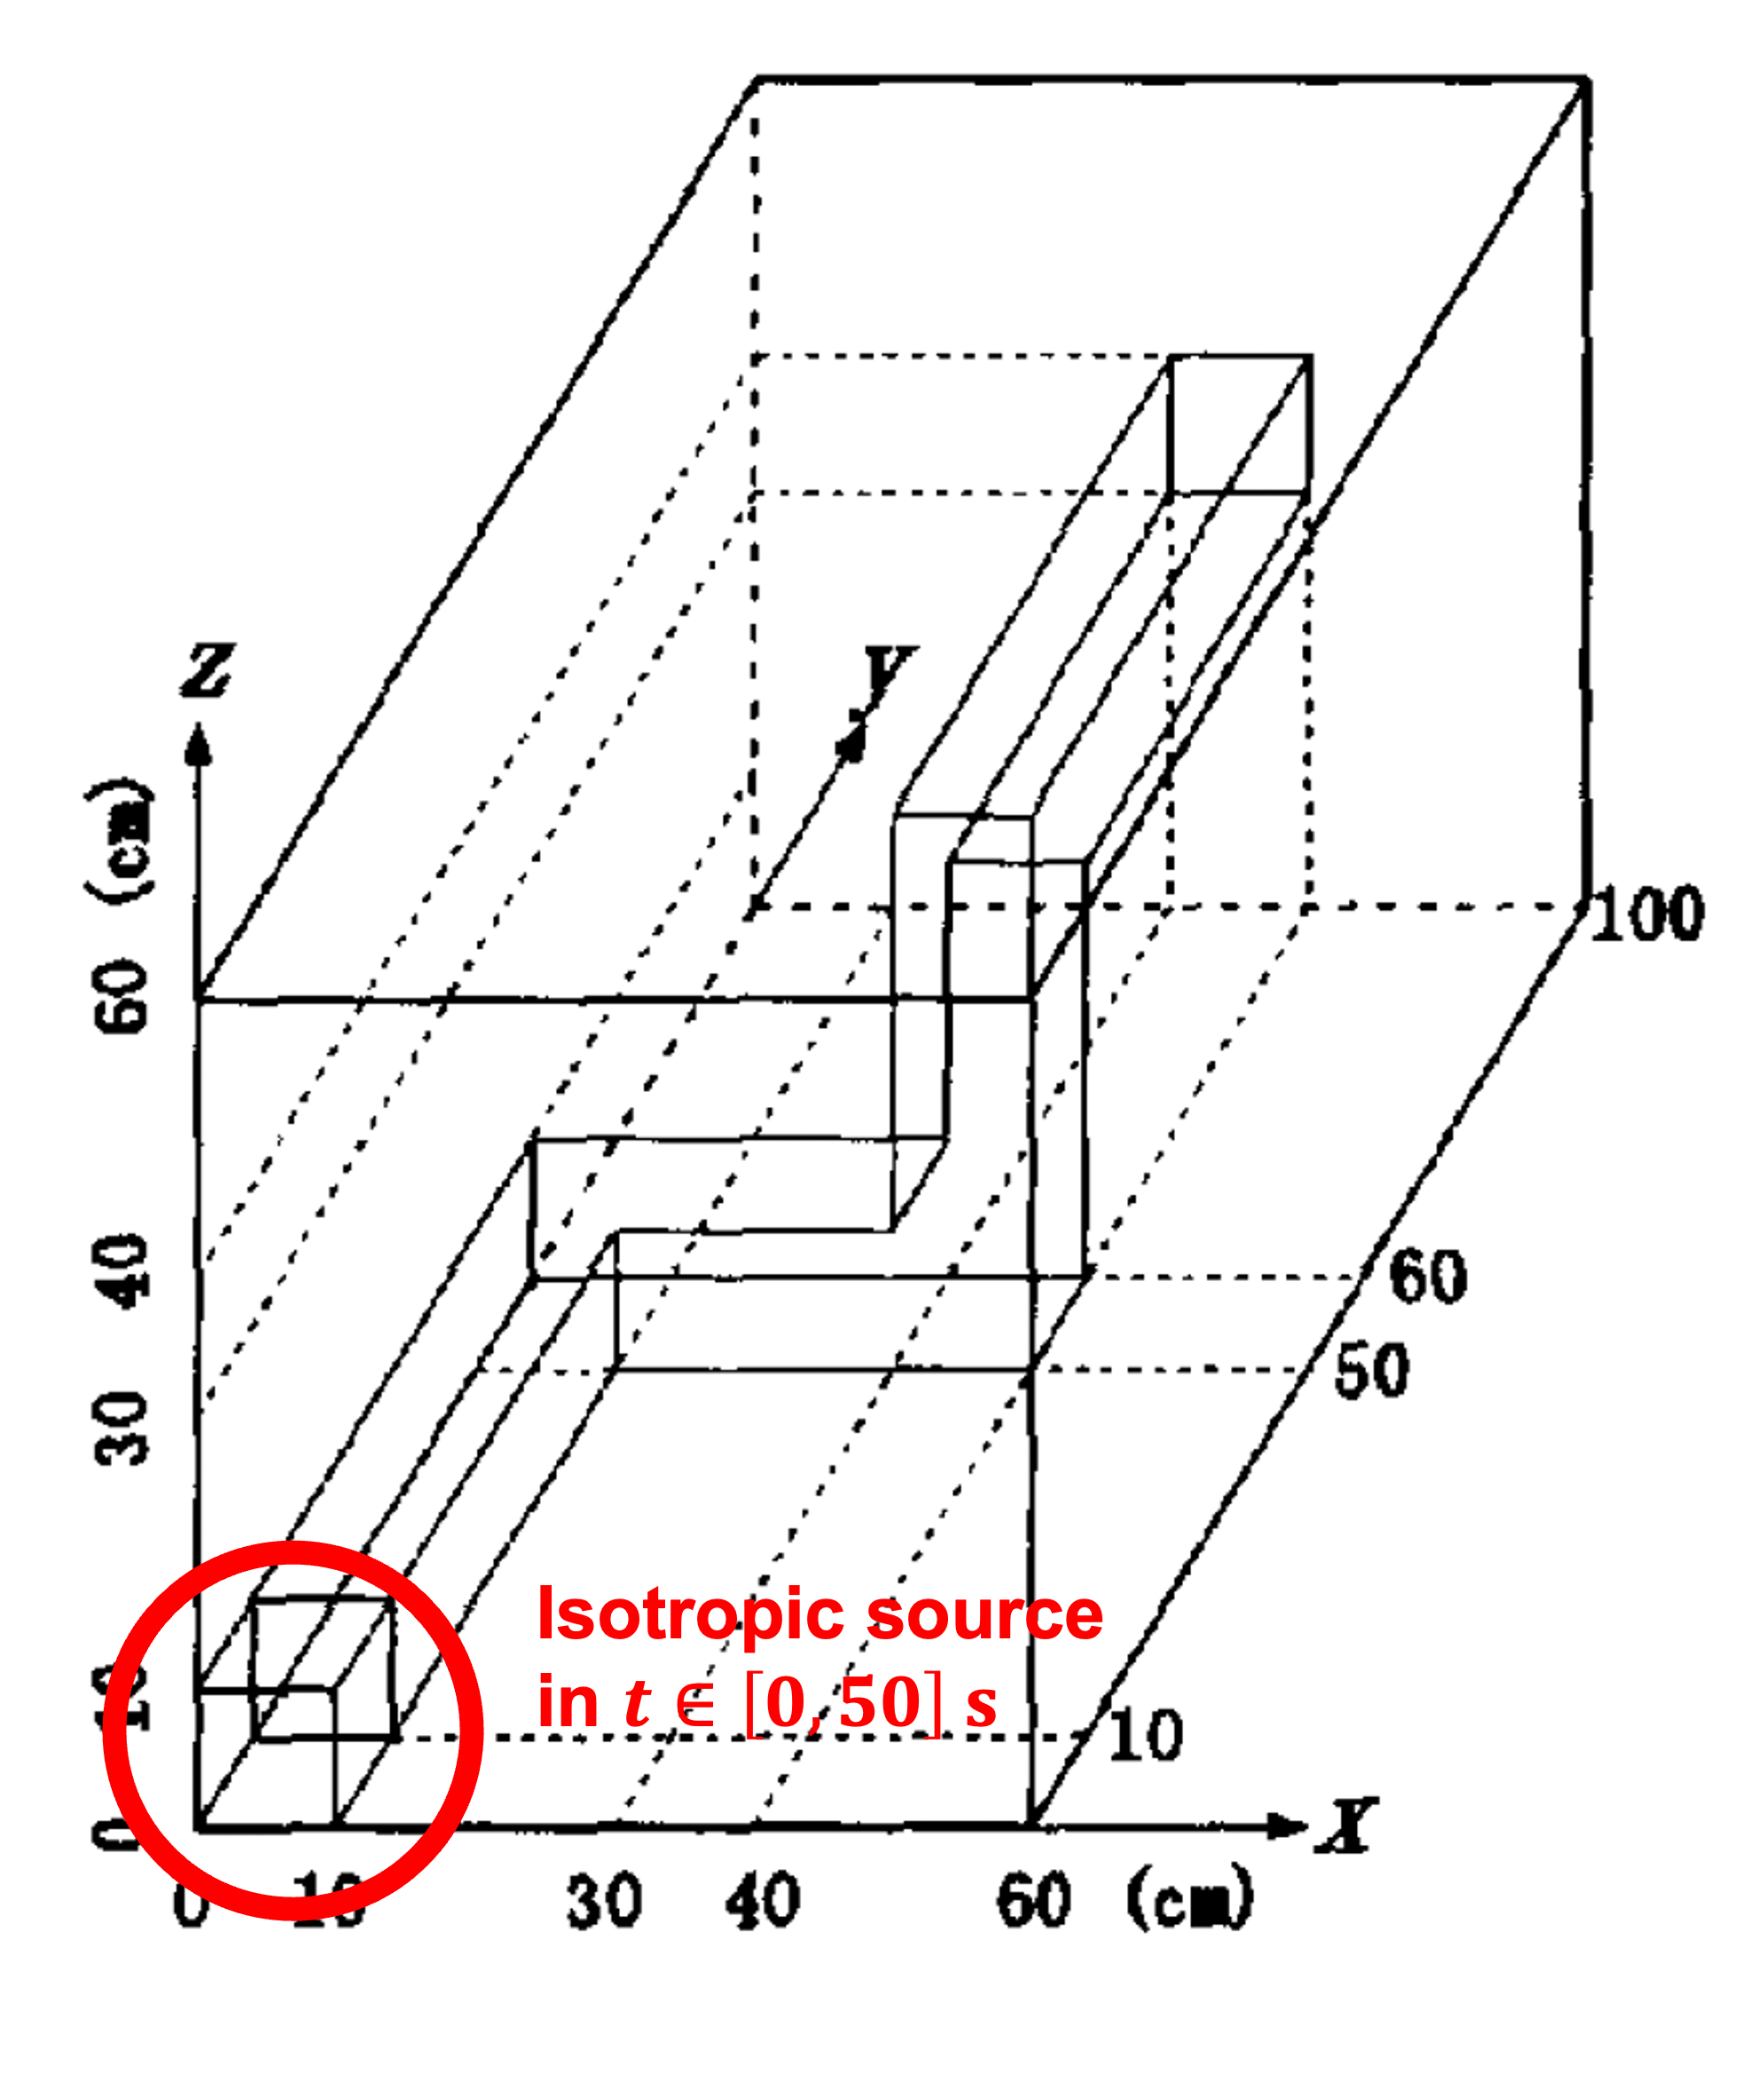
\includegraphics[width=.4\textwidth]{figures/results/kobayashi_problem.png} \hspace{1cm}
    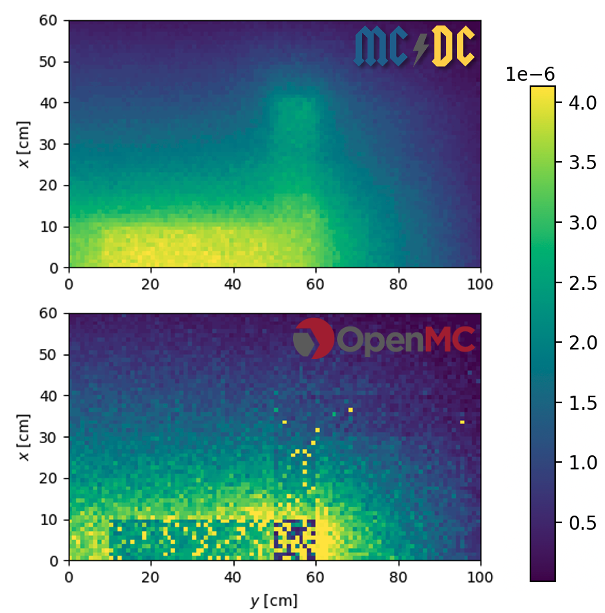
\includegraphics[width=.5\textwidth]{figures/results/koby_mcdcopenmc.png}
    \caption{Left: Kobayashi problem schematic. Right: Time and space averaged scalar flux solution to the Kobayashi problem run with \num{1e9} particle histories from MC/DC (top) and OpenMC (bottom).}
    \label{koby-problem}
\end{figure*}

Figure~\ref{performance_results} at left shows the runtime results of MC/DC compared with OpenMC on a single node of the Quartz supercomputer (two socket 18-core Intel Xeon E5-2695 v4) at Lawrence Livermore National Laboratory (LLNL).
Caching in MC/DC was enabled for these results, meaning there is no JIT compilation overhead.
We examine the impact of a variance reduction technique called implicit capture \cite{lewis_computational_1984}, which is supported in both codes.
OpenMC is about 20 times faster than MC/DC for this problem with implicit capture.
Without implicit capture that performance gap falls to 12 times.
This performance gap is due to OpenMC's tracking algorithm, which does not stop particles at mesh crossing events as MC/DC currently does.
OpenMC is currently limited to the use of the collision estimator to estimate the scalar flux spatial distribution in time-dependent simulation, whereas MC/DC uses the track length estimator \cite{lewis_computational_1984}, which is computationally more expensive but yields better statistics.
This is shown in figure~\ref{koby-problem} at bottom right where OpenMC's result has tally cells with a poorly converged solution (displaying as yellow spots) and MC/DC's (top right) doesn't.
Work is ongoing to implement this particle stop command.
When this is enabled, we suspect the performance gaps for this problem will close substantially between MC/DC and OpenMC.

\begin{figure*}[h]
    \centering
    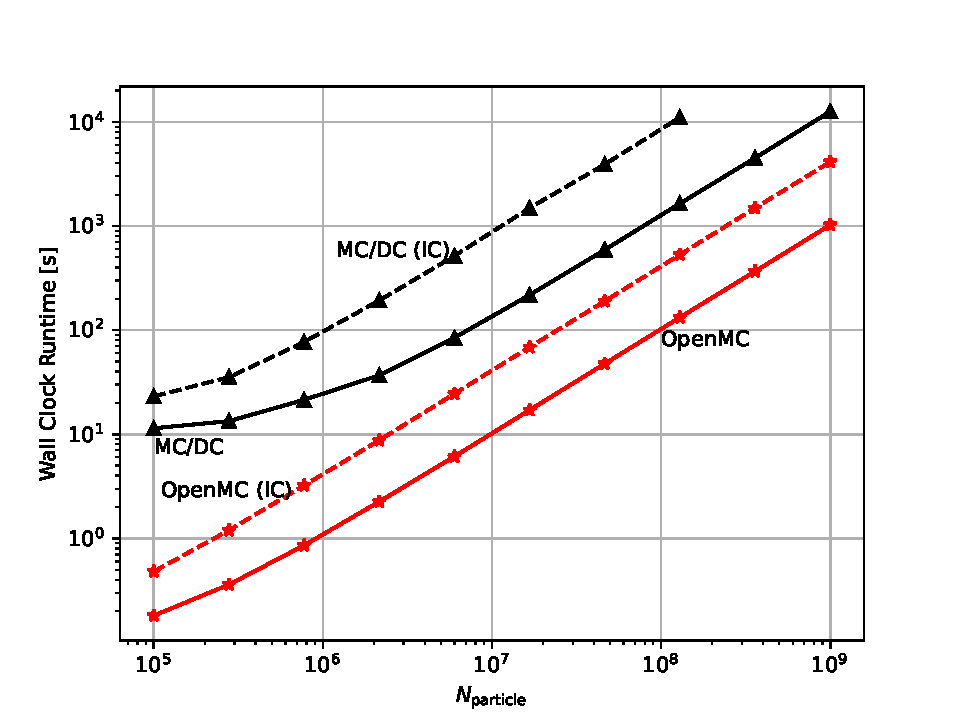
\includegraphics[width=.49\textwidth]{figures/results/code_comparisons.pdf}
    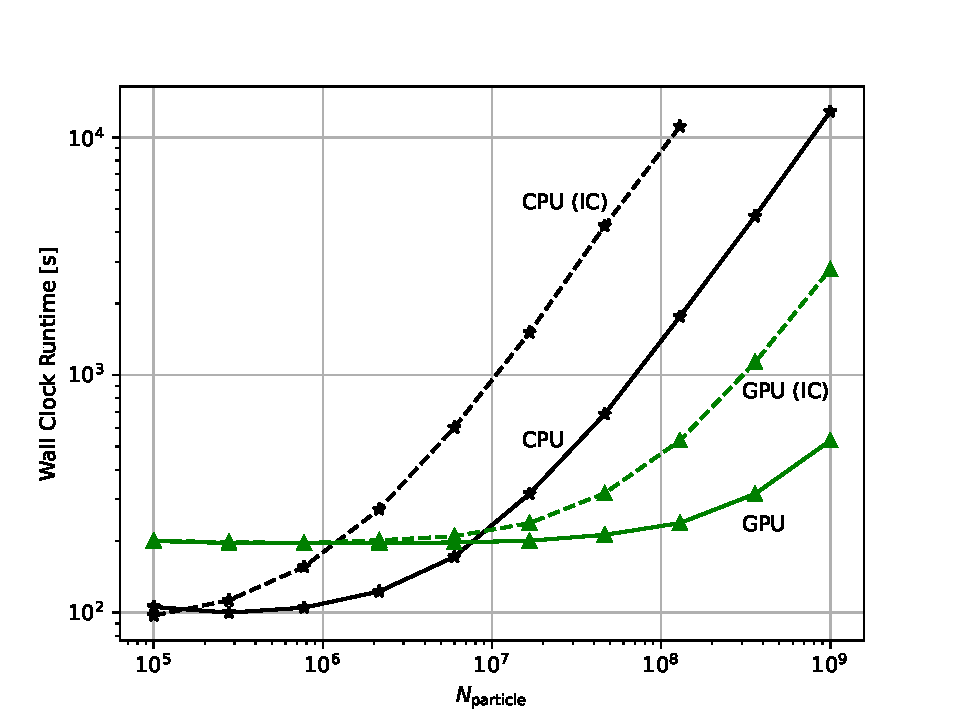
\includegraphics[width=.49\textwidth]{figures/results/mcdc_comparisons.pdf}
    \caption{Left: Wall clock runtime of the Kobyashi problem over particle counts with and without implicit capture (IC) between cached MC/DC (black) and OpenMC (red). 
    Right: Wall clock runtime of the Kobyashi problem over particle counts in uncached MC/DC CPU (black) and GPU (green) modes.}
    \label{performance_results}
\end{figure*}

While these performance results are promising more work is needed to explore MC/DC's (and by extension the software engineering scheme using Numba) performance on modern hardware.
I propose examining the performance of MC/DC more stringently on GPU accelerators including thru the use of code profilers when available.
Also expanding the performance analysis of MC/DC on GPUs to other problems of interest (Dragon burst experiment, C5G7, etc.), other currently enabled GPU types (AMD), and multi-GPU computations.
These initial investigations go to answer research question 1.

\subsection{Hybrid delta tracking in MCATK}

Three experiments where used to confirm that the hybrid delta tracking scheme converged to the expected solution. This was done  via code-to-code comparison
K-eigenvalue simulations were started with 100 inactive cycles before 500 active ones using \num{1e5} particles in each cycle.
Table \ref{table:runtime} shows the performance increase when hybrid-delta tracking is enabled.
The differences in eigenvalue between simulations with and without the hybrid-delta tracking algorithm are all within 1.12 standard deviations. This table also shows a significant speed-up in the over all solve time of MCATK with delta tracking incurring between a 1.54--1.75$\times$ speed-up.

\begin{table}[!htb]
  \centering
  \caption{Benchmark results: where ${\Delta \sigma}$ is the difference in number of standard deviations of ${k_{\text{eff}}}$ between the standard algorithm and hybrid-delta tracking.}
  \label{table:runtime} 
  \begin{tabular}{@{}c c c c c c@{}} \toprule
    Benchmark & MCATK & MCATK & $k$ & $\Delta \sigma$ & speed-up\\
               & Surface (s)  & Hybrid-Delta (s) &  & &\\ \midrule
    \ Godiva Case 5 & 16900 &  10987 & 0.99736 &  -0.747 & 1.54 \\
    \ MUSiC Case 8  & 23937 &  14832 & 0.99970 &  0.130 & 1.61 \\
    \ MUSiC Case 9  & 22649 &  12973 & 0.99929 &  -1.105 & 1.75 \\ 
    \bottomrule
  \end{tabular}
\end{table}


\begin{table}[!htb]
  \centering
  \caption{Benchmark results: where $\Delta \sigma$ is the difference in number of standard deviations of the $\alpha$-eigenvalues between standard algorithm and hybrid-delta tracking.}
  \label{table:runtime_trans} 
  \begin{tabular}{{@{}c c c c c c@{}}} \toprule 
    Benchmark & MCATK            & MCATK         & $\alpha_{\text{avg}}$ & $\Delta \sigma$ & speed-up\\
               & Surface (s)  & Hybrid-Delta (s) & &                 &\\ \midrule
    \ Godiva Case 5 & 2689 &  2168 & \num{-3.54e-3} &  \num{-1.91} & 1.24 \\
    \ MUSiC Case 8  & 4352 &  2665 & \num{-1.26e-3} &  \num{-0.76} & 1.63 \\
    \ MUSiC Case 9  & 4440 &  2786 & \num{-1.02e-3} &  \num{-2.75} & 1.59 \\ 
    \bottomrule
  \end{tabular}
\end{table}

To compute error between tracking schemes in fixed source simulations we used the estimates of the $\alpha$-eigenvalue computed using MCATK's time-dependent algorithm.
The benchmarks were started at \SI{0}{\second} and ran to \SI{500e-8}{\second} with a time step of $\Delta t =$ \SI{1e-8}{\second}.
The particle population was combed between every time step up or down to \num{1e5} particles. 
Table \ref{table:runtime_trans} shows less speed-up then for k-eigenvalue computations (only between 1.24$\times$ and 1.63$\times$) but still significant for minimal alterations to a production code. This table also shows the average $\alpha$-eigenvalues method within three standard deviations.

Hybrid-delta tracking on a structured mesh improves run time in large and materially complex simulations like the ones we benchmarked: 1.5--1.75$\times$ speed-up for k-eigenvalue and 1.2--1.6$\times$ speed-up for fixed source problems.
FOMs where not produced as part of the work in MCATK.
The speedup in MCATK was entirely due to the elimination of extra cross section lookups in an otherwise standard surface tracking algorithm with a track length estimator.
These conclusions go to answer research question 5.

These initial investigations in MCATK gives confidence that when implemented in MC/DC we will also see performance improvements.
When moving towards an implementation in MC/DC we expect a potential speedup (due to eliminated distance to surface computations) but more marginal speedup in materially complex problems.
I do expect that adding  a track length estimator to make the variance very small.
Work in MC/DC is ongoing beginning with the majorant computation functionality.